\section{Demonstration and Testing}
\label{demo}

\subsection{Demonstration by Walkthrough}

This section describes a walkthrough of two user stories the team developed based on our requirements, to demonstrate the primary features currently implemented in the finished prototype system. 

\subsubsection{Complete Decomposition Scenario}
\label{Scenario1}

\begin{figure}
\centering
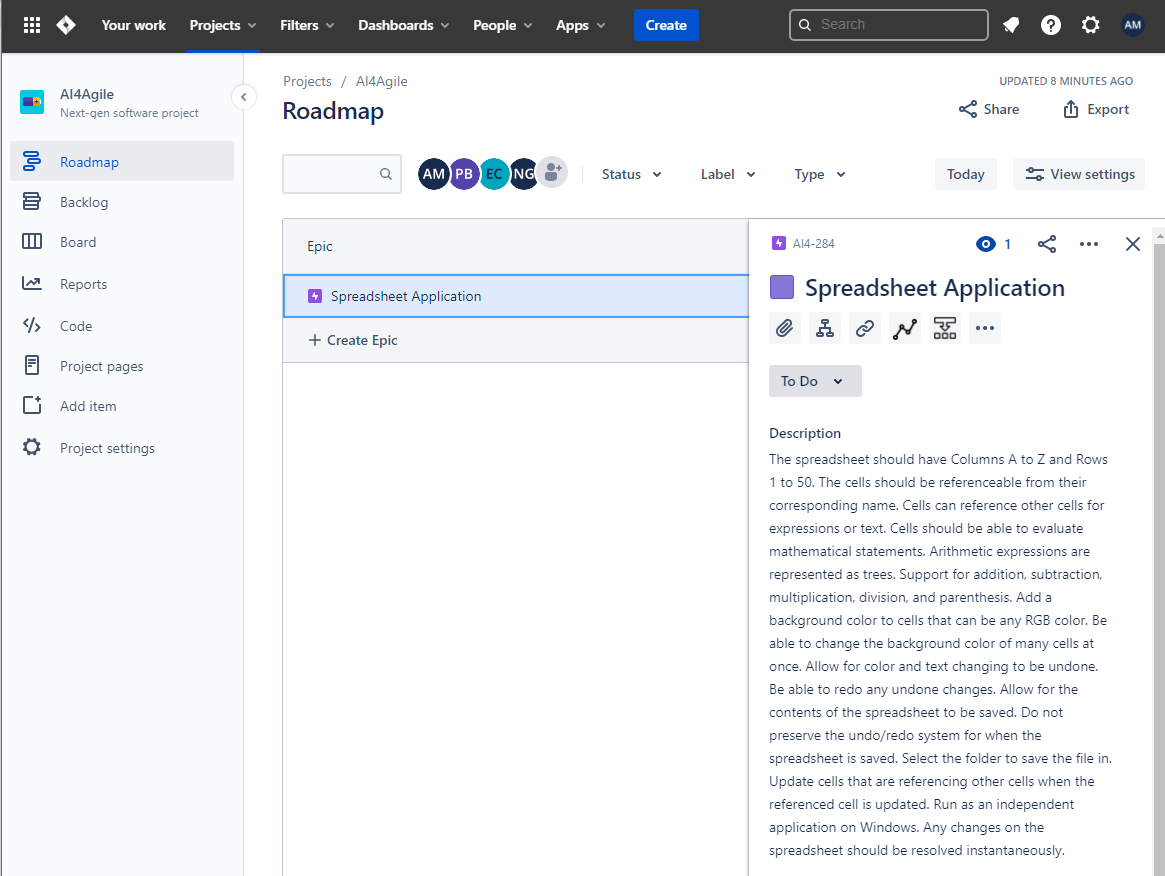
\includegraphics[width=\textwidth,keepaspectratio]{./figure/Scenario1Figure1.png}
\caption{Overall view of Jira Roadmap with Decompose Epic button in focus}
\label{fig:Scenario1Figure1}
\end{figure}

Frank is a software requirements analyst, and he wants to speed up the process of breaking an epic full of requirements into smaller user stories. For this purpose, he installs the AI4Agile plugin to Jira. Frank creates a new epic, puts the requirements for his Spreadsheet Application in as plaintext sentences, and clicks the Decompose Epic button (Fig. \ref{fig:Scenario1Figure1}).

\begin{figure}[ht]
\begin{subfigure}{.5\textwidth}
\centering
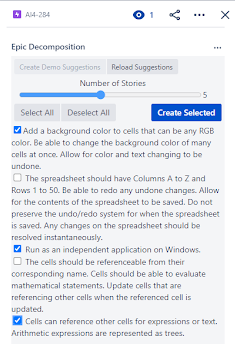
\includegraphics[width=.8\linewidth,keepaspectratio]{./figure/Scenario1Figure2.png}
\caption{Generated User Story Suggestions}
\label{fig:Scenario1Figure2}
\end{subfigure}
\begin{subfigure}{.5\textwidth}
\centering
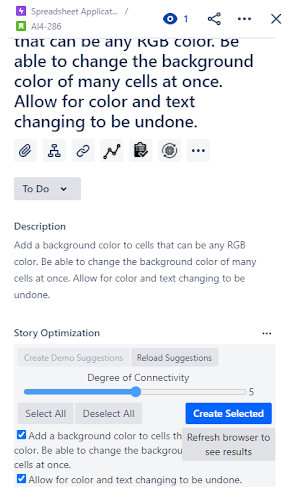
\includegraphics[width=.8\linewidth,keepaspectratio]{./figure/Scenario1Figure3.png}
\caption{User Story Optimization Suggestions}
\label{fig:Scenario1Figure3}
\end{subfigure}
\caption{User Story Suggestions Views}
\end{figure}

Now, Frank looks at the suggestions the AI came up with (Fig. \ref{fig:Scenario1Figure2}). If he decides he doesn’t like any of these suggestions, he can click the Ignore All button to go back to his Spreadsheet Application epic. If Frank wants more or fewer stories, he can adjust the value on the slider and it will refresh the results. To edit a story, he can click on its text box, then save or cancel those edits. To ignore a story suggestion entirely, he can leave its box unchecked. Once Frank is happy with his resulting user story or the set of stories he wants, he clicks Create Selected. 

After refreshing the webpage, the newly created user stories that Frank approved are visible under the heading of the Spreadsheet Application epic.

If Frank wants to continue the process of breaking up epics, he can go into one of the user stories and click Optimize User Story (Fig. \ref{fig:Scenario1Figure3}). Depending on the size of the user story already, it might be broken down into multiple smaller stories, or left alone if it’s already optimized.

Once the Story Optimization Suggestions are generated, Frank has the same options as with the previous stories: to select or deselect stories via the checkboxes, make edits, or ignore all suggestions. In addition to those options, Frank can choose to adjust the connectivity slider to change how closely related items need to be in order to stay with the same story.  

Now there are five user stories, since Story 4 was optimized into two separate stories. To continue the decomposition process, Frank opens a story and clicks Generate Tasks (fig. \ref{fig:Scenario1Figure2}).

\begin{figure}
\begin{subfigure}{.5\textwidth}
\centering
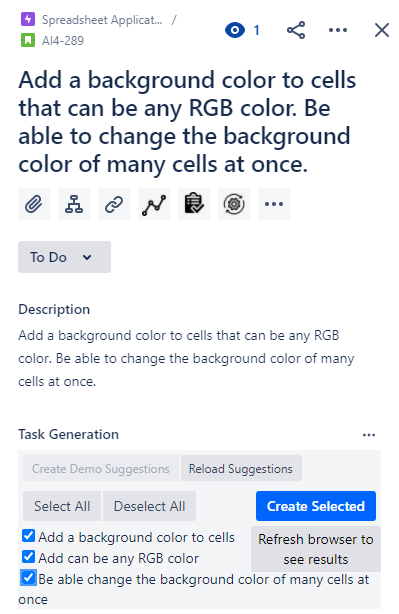
\includegraphics[width=.8\linewidth,keepaspectratio]{./figure/Scenario1Figure4.png}
\caption{Task Suggestions page}
\label{fig:Scenario1Figure4}
\end{subfigure}
\begin{subfigure}{.5\textwidth}
\centering
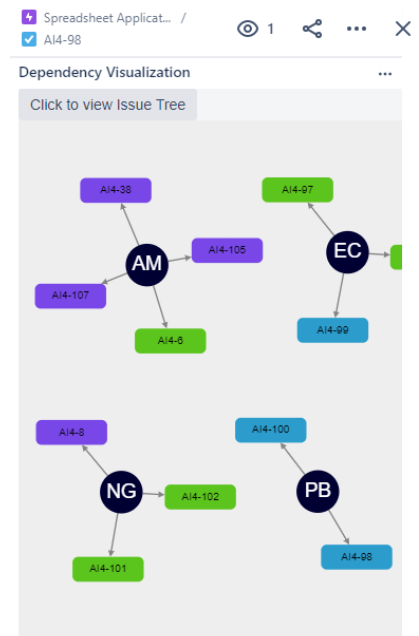
\includegraphics[width=.8\linewidth,keepaspectratio]{./figure/Scenario2Figure2.png}
\caption{Developer cluster graph on a selected task}
\label{fig:Scenario2Figure2}
\end{subfigure}
\caption{Task suggestions and Cluster Graph}
\end{figure}

As before, the options include selecting or deselecting individual suggestions, editing, and ignoring all suggestions. Once he’s happy with the tasks, he clicks Create Selected.

\begin{figure}
\centering
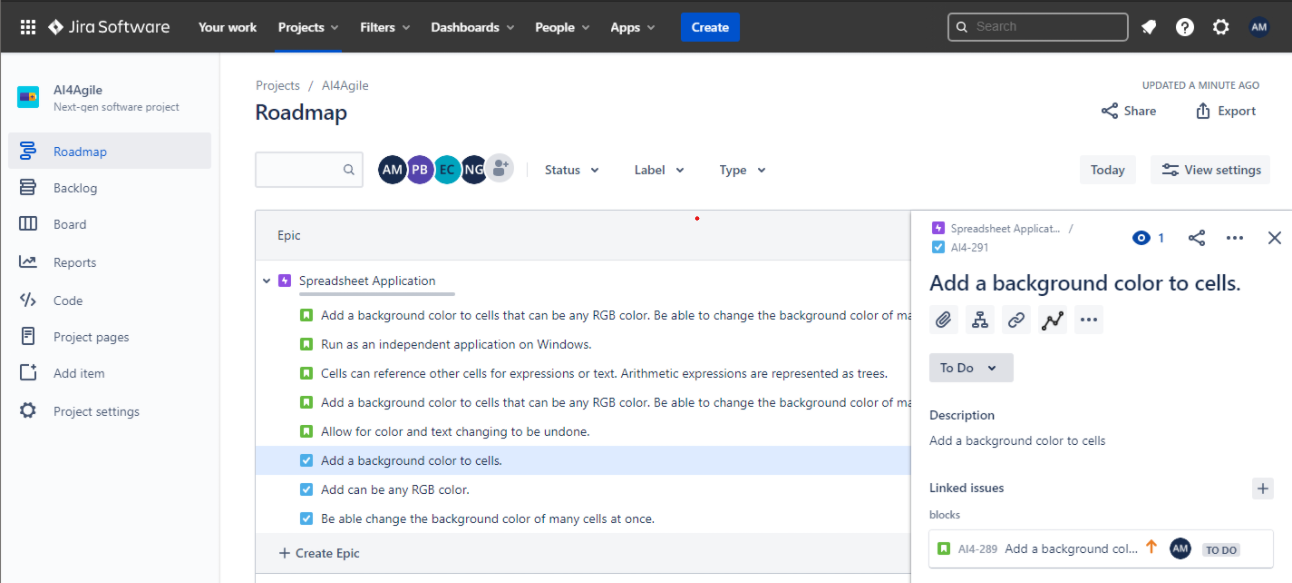
\includegraphics[width=\textwidth,keepaspectratio]{./figure/Scenario1Figure5.png}
\caption{View of newly created tasks for one fully decomposed user story}
\label{fig:Scenario1Figure5}
\end{figure}

The tasks have now been created, and linked to their parent story to indicate a blocking relationship. All Frank had to do was make some decisions and maybe edits, and now he’s got one story fully decomposed (Fig. \ref{fig:Scenario1Figure5}).

\subsubsection{Relationship Visualization Scenario}
\label{Scenario2}

\begin{figure}
\centering
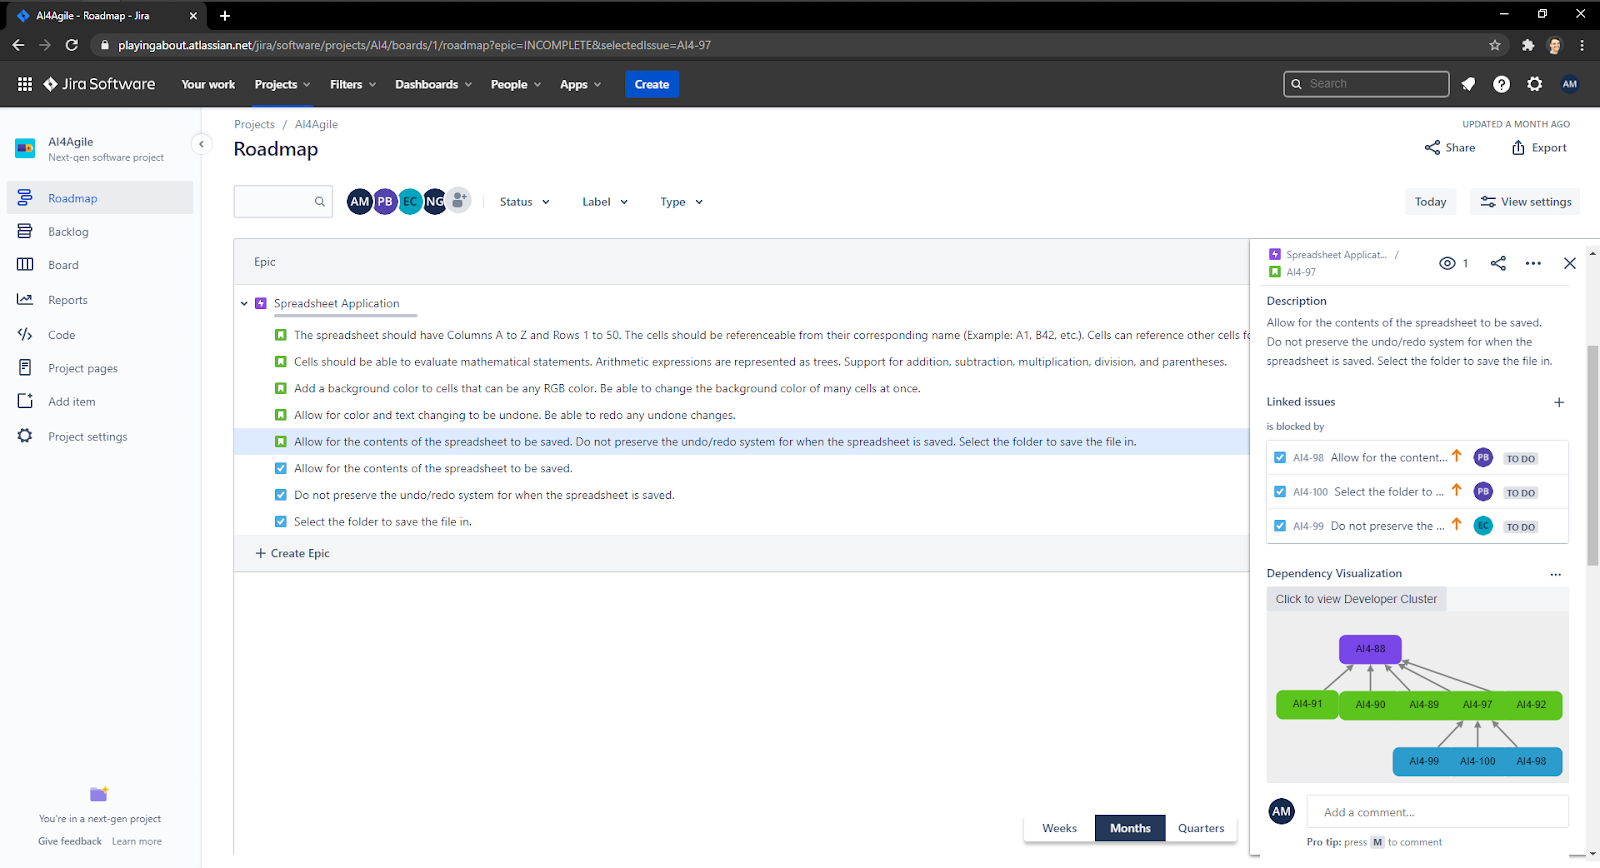
\includegraphics[width=\textwidth,keepaspectratio]{./figure/Scenario2Figure1.png}
\caption{A zoomed out view of navigating to the issue relationship graph}
\label{fig:Scenario2Figure1}
\end{figure}

Madison is a scrum master, and she wants to take a closer look at some of the tasks to make sure the developer assignments make sense. To do this, she uses the AI4Agile Issue Relationship Graph feature by navigating to a certain epic, user story, or task, and finding the graph portion (Fig. \ref{fig:Scenario2Figure1}). Now, Madison can see all the available relationships between the task she has selected and other tasks, stories, and the epic they came from. She is better able to decide whether the team members she assigned to these pieces make sense given the relations between them.

For an alternate view of the relationships, Madison can use the Click to view Developer Cluster button (Figure. \ref{fig:Scenario2Figure1}) to see what the current assignments and workload look like for her team (Figure. \ref{fig:Scenario2Figure2}). If she wants to go back to the previous graph view, the Click to view Issue Tree button is in the top left corner.

\subsection{Testing}

The application is primarily composed of individual web panels integrated into Jira’s existing User Interface. As a result, each web panel was able to be created, tested, and reviewed independently from Jira Cloud. The isolation was used to conduct input and output testing but the modules were generally tested within the context of Jira to ensure that the user experience is seamless between our integrated app and the existing Jira Cloud platform.

The rest of functional testing was performed on component and integration levels. Component testing was separated into two categories: text processing and relationship visualization.

We based the testing of the text processing component upon results from three categories of inputs: ideal, disjoint, and semi-ideal. Ideal inputs were those where all information belonged to clear categories. Disjoint inputs were those where all information fell completely within separate categories. Semi-ideal inputs had both outlier pieces of information and information that distinctly can be clustered with other info. Disjoint inputs were used to evaluate edge case usages of the tool. To represent the average case, semi-ideal inputs were used since natural language understanding from a vector perspective is ambiguous without context.

For integration testing, all possible user paths were explored as each text process could be done independently or sequentially. For example, a user can complete the entire process by entering by decomposing an epic, optimizing the generated stories, and then generate tasks from the optimized stories. However, a user may choose to only optimize stories that were manually entered and then go on to generate tasks from the optimized stories. 
